\documentclass[a4paper,10pt, twocolumn]{article}
\usepackage[a4paper,top=2cm,bottom=3cm,left=2cm,right=2cm,footskip=0.8cm]{geometry}
\usepackage{lipsum}
\usepackage{graphicx}
\usepackage{float}
\usepackage{caption}    % Para personalizar legendas, opcional
\usepackage{xcolor}
\usepackage{fancyhdr}
\usepackage{helvet}
\usepackage{}
\usepackage{multicol}
\usepackage{titlesec}     % Para personalizar \section
\usepackage[style=ieee, sorting=nty, language=portuguese]{biblatex}
\definecolor{grayFEI}{HTML}{7F7F7F}
\usepackage{paracol} % no preâmbulo
\usepackage{indentfirst}  % Indenta o primeiro parágrafo
\setlength{\parindent}{2em}  % Aumenta a indentação para 2em (pode ser ajustado
\titlespacing*{\section}{0pt}{*0}{0pt}
\usepackage{ragged2e}


%-------------------------- ESTILOS NÃO ALTERAR ------------------------------------------------%
% Estilo para legendas de figura e tabela
\captionsetup[figure]{
  labelfont={color=azulFEI, bf, small, sf}, % "Figura" azul, negrito, Arial-like
  textfont={small, sf},                    % Texto da legenda em Arial-like
  font=footnotesize,                       % Tamanho aproximado de 9pt
  labelsep=period,                         % "Figura 1." e não "Figura 1:"
  name=Figura,                             % Tradução para "Figura"
  justification=raggedright,              % Alinhado à esquerda
  singlelinecheck=false                   % Garante alinhamento mesmo em uma linha
}

\captionsetup[table]{
  labelfont={color=azulFEI, bf, small, sf},
  textfont={small, sf},
  font=footnotesize,
  labelsep=period,
  name=Tabela,
  justification=raggedright,
  singlelinecheck=false
}

% Formatação section e subsection
\titleformat{\subsection}
  {\color{grayFEI}\normalfont\fontfamily{phv}\selectfont\itshape\fontsize{10}{12}\selectfont}
  {\thesubsection.}{0.2em}{}
\renewcommand{\thesubsection}{\Alph{subsection}}

\titleformat{\section}
  {\color{azulFEI}\normalfont\fontfamily{phv}\selectfont\bfseries\fontsize{11}{13}\selectfont} % Fonte Helvetica, tamanho 11pt, negrito
  {\thesection.}{0.2em}{}
\renewcommand{\thesection}{\Roman{section}}
\titlespacing*{\section}
{0pt}{10pt}{0pt}

%Formatação Título
\newcommand{\inovatitle}[1]{%
  \noindent{\fontsize{18}{20}{\helvet{\textbf{\textcolor{azulFEI}{#1}}}}}\vspace{25pt}
}

%Formatação Autores
\newcommand{\autores}[1]{
  \helvet{\fontsize{11}{20}\selectfont\textbf{\textit{#1}}}
}
\newcommand{\orientador}[1]{
  \helvet{\fontsize{11}{20}\selectfont\textbf{\textit{#1}}}
}
\newcommand{\filiacao}[1]{
  \helvet{\fontsize{10}{20}\selectfont{\textit{#1}}}
}
\newcommand{\email}[1]{
  \helvet{\fontsize{10}{20}\selectfont{\textit{#1}}\newline}
}
\newcommand{\resumo}[1]{%
\vspace{15pt}
  \noindent
  {\helvet{\fontsize{12}{20}\selectfont\textbf{\textcolor{azulFEI}{Resumo:}}}} %
  \justifying #1 %
  \newline
}

\newcommand{\keyword}[1]{
  \noindent\helvet{\fontsize{12}{20}\selectfont\textbf{\textcolor{azulFEI}{Palavras-chaves:}}} #1  \vspace{25pt}
}

\renewcommand{\thetable}{\Roman{table}}


% Define a cor azul específica (exemplo: azul FEI)
\definecolor{azulFEI}{HTML}{0070C0} % substitua pelo código que quiser

%Formatação Cabeçalho e rodapé
\setlength{\headsep}{1cm}
\newcommand{\helvet}[1]{{\fontfamily{phv}\selectfont #1}}
\pagestyle{fancy}
\fancyhead{} % limpa cabeçalho
\renewcommand{\headrulewidth}{0.3pt} % ← ATIVA a linha (espessura ajustável)
\setlength\headheight{1.2cm}
\lhead{
\includegraphics[width=4.97cm, height=1cm]{logoinova.png}}
\rhead{\helvet{1º semestre/2025}}

\fancyfoot{} % limpa rodapé
\lfoot{
  \fontfamily{phv}\fontsize{8}{10}\selectfont
  Anais dos Trabalhos de Conclusão de Curso do Centro Universitário FEI, São Bernardo do Campo – SP\\
  \vspace{-4pt}\rule{\textwidth}{1pt} % ← linha abaixo do texto do rodapé
}
\rfoot{\fontfamily{phv}\fontsize{8}{10}\selectfont \thepage}

%-------------------------------- FIM ESTILOS ---------------------------------------------------%

%Adicionar a bibliografia
\addbibresource{referencias.bib}

\begin{document}

\setlength{\columnsep}{20pt}
\twocolumn[%
\begin{@twocolumnfalse}

\raggedright{

\inovatitle{Estudo e Implementação de um Sistema de Segmentação Semântica para Ambientes Off-Road}

\autores{Henrique Finatti$^1$, Mateus Marana$^1$, Tiago Fagundes$^1$}

\filiacao{$^1$Ciência da Computação - campus São Bernardo do Campo}

\email{unifhtrebbi@fei.edu.br, unimassuena@fei.edu.br, uniftsantos@fei.edu.br}

\orientador{Orientador: Pr. Dt Isaac Jesus da Silva}

\filiacao{Departamento de Ciência da Computação / Engenharia Elétrica, Centro Universitário FEI}

\email{isaacjesus@fei.edu.br}

\resumo{
  O campo da segmentação semântica tem crescido significativamente com os avanços da visão computacional,
  e sua aplicação em ambientes off-road é um dos grandes desafios da área devido a dificuldade de identificar caminhos
  e diferenciar diferentes obstáculos presentes nas trilhas.
  Diante desse cenário esse trabalho apresenta um modelo de segmentação semântica
  desenvolvido com a arquitetura DeepLabV3+, proposta pela Google, utilizando a ResNet101 como backbone. O modelo será
  treinado com diversos datasets encontrados em artigos recentes na área da segmentação semântica aplicada em ambientes off-road.
  O objetivo deste trabalho é desenvolver e treinar o modelo para obter bons resultados no dataset YAMAHA, conhecido como
  um dos datasets mais desafiadores para segmentação. Além disso, pretendemos aplicar o modelo na segmentação de imagens
  e vídeos de competições Baja realizadas pela equipe da FEI, utilizando como métrica principal IoU (Intersection over Union)
}

\keyword{Segmentação Semântica, Off-Road, DeepLabV3+, YAMAHA, FALTA 2/3 PALAVRAS}
}

\end{@twocolumnfalse}
]



\section{Introdução}

% Explicação da segmentação
% (P)
A área da visão computacional tem impactado diretamente os avanços do campo da segmentação semântica, quando falamos sobre essa vertente em ambientes off-road os desafios são múltiplos devido a bordas indeterminadas nas trilhas, variedade de obstáculos e mudanças frequentes em diferentes épocas e estações do ano.
% (E)
% Pesquisar artigo de evidência da dificuldade da segmentação semântica em off road. (Tiago)
% (E)
Com base nos artigos citados acima o mesmo modelo de segmentação teve mais dificuldade para segmentar ambientes off-road comparado a ambientes urbanos, mesmo tendo um treinamento parecido.
% (L)
Dessa forma, o reconhecimento de vias não urbanas ainda é um desafio a ser explorado.

% Explicação da CNN
% (P)
As Redes Neurais Convolucionais (CNNs) são amplamente utilizadas em tarefas de visão computacional devido à sua capacidade de extrair características relevantes de imagens, tornando-se fundamentais para aplicações como segmentação semântica.
% (E)
% Ainda precisamos de algum artigo nessa bomba
Estudos recentes demonstram que arquiteturas baseadas em CNNs, como DeepLabV3+, apresentam alto desempenho em tarefas de segmentação.
% (E)
Essa capacidade é especialmente importante em cenários off-road, onde a área visual possui muitos elemento e as fronteiras entre classes são mais difíceis de interpretar, exigindo modelos mais capacitados para segmentar as imagens.
% (L)
Dessa forma, esse trabalho, faz uso de uma arquitetura baseada em CNN, especificamente o modelo DeepLabV3+, visando obter uma segmentação mais precisa.

% Explicação do dataset
% (P)
A escolha e a diversidade dos datasets utilizados no treinamento são muito relevantes para o desempenho dos modelos de segmentação, especialmente em cenários off-road.
% (E)
% Talvez pegar um artigo que utilize uma mistura de datasets, o primeiro da lista monta um dataset sintético baseado no PASCAL VOC, talvez seja bom
% (E)
Nesse contexto, este trabalho utiliza uma coletânea de datasets que foram utilizados em estudos recentes da área, incluindo o dataset YAMAHA, reconhecido pela sua alta complexidade, variabilidade de cenários e dificuldade na definição de classes.
% (L)
Dessa forma, a utilização de múltiplos datasets, com destaque para o YAMAHA, proporciona um melhor treinamento do modelo, permitindo avaliar seu desempenho em diferentes condições.

\section{Formatação da página}
As margens da folha estão definidas na Tabela I. O trabalho deve conter resumo; introdução; objetivos, metodologia; resultados e conclusões além de eventuais referências bibliográficas. Seções adicionais podem ser incluídas, caso necessário.

O corpo do trabalho deve ser escrito com caracteres de tamanho 10, sem linhas em branco separando os parágrafos. Em cada novo parágrafo, o início da primeira linha deve ser deslocado em 0,5 cm, conforme modelo. Cabeçalho e rodapé não devem ser alterados.

As referências devem ser indicadas entre chaves [1] ao longo do texto e descrito no final do artigo citando: nomes dos autores (pode ser abreviado, no máximo três nomes e caso tenha mais nomes usar o et. al.), nome da revista, volume, ano da publicação e página ou nome do livro, editor e ano de publicação.
Por exemplo: em \cite{10.1145/3716895.3716981} foram realizados muitos testes, alcançando uma acurácia de 100\%. Já em \cite{10.1145/3593239} não obtiveram resultados satisfatórios.

\section{Figuras, tabelas e equações}

\subsection{Figuras}
As figuras devem ser centralizadas, e as legendas devem ser numeradas sequencialmente, alinhadas à esquerda na parte inferior, conforme exemplo apresentado, usando fonte Arial tamanho 9. O tamanho da figura e das letras dentro das figuras deve estar legível. Cores podem ser utilizadas, desde que apresentem boa resolução. As figuras devem ser citadas no texto, por exemplo, a Figura \ref{fig:minhafigura-coluna} apresenta um gráfico.

\begin{figure}[h!] % ← precisa do pacote float
\centering
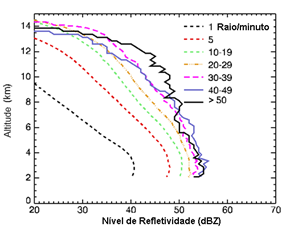
\includegraphics[width=0.8\columnwidth]{exemplofig.png}
\caption{Legenda da figura dentro da coluna}
\label{fig:minhafigura-coluna}
\end{figure}

\subsection{Tabelas}
As tabelas devem ser referenciadas sequencialmente, com a legenda posicionada na parte superior da mesma e alinhada à esquerda, usando fonte Arial tamanho 9.\textbf{ O texto nas células da tabela deve ser centralizado. Usar o comando $|c|$} Elas devem ser citadas no texto, por exemplo a Tabela \ref{tab:exemplo} apresenta as informações das margens.

\begin{table}[H]
\caption{Legenda da tabela, precisa ser intuitivo.}
\label{tab:exemplo}
\begin{tabular}{|c|c|}
\hline
\textbf{Margem} & \textbf{Tamanho (cm)} \\ \hline
Superior & 2,0 \\ \hline
Inferior & 2,0 \\ \hline
Esquerda & 2,0 \\ \hline
Direita & 2,0 \\ \hline
Coluna & 1,0 \\ \hline
\end{tabular}
\end{table}


\subsection{Equações}
Caso seja necessário incluir equações, estas devem ser apresentadas em itálico, alinhadas à esquerda, e numeradas no lado direito entre parênteses.
\begin{equation}
    W= \theta_1 - \theta_2
\end{equation}

\section{Conclusões}
Destaque os principais resultados alcançados e contribuições do trabalho desenvolvido.

\section{Referências}
\printbibliography[heading=none]

\section*{Agradecimentos}
A seção de agradecimentos é opcional.\textbf{ Autores (incluindo o professor orientador) não devem ser incluídos nos agradecimentos. }


\end{document}